\documentclass[a4paper, 12pt]{article}  %set doc type and font size
\usepackage{fontspec}                   %allow setting fonts
\usepackage{xeCJK}         
\usepackage{amsmath}
\newtheorem{theorem}{Theorem}
\setCJKmainfont{Noto Sans CJK SC}             %call chinese package xeCJK
% \setmainfont{Times New Roman}           %set English font

% \XeTeXlinebreaklocale "zh"
% \XeTeXlinebreakskip = 0pt plus 1pt


\usepackage{algorithm}
\usepackage[noend]{algpseudocode}

\usepackage{mdframed}    % for frames
\usepackage{xcolor}      % for colors

\usepackage{amsthm}

\usepackage{graphicx}

\usepackage[most]{tcolorbox}
\tcbset{
  theorem style/.style={
    enhanced,
colback=blue!2!white,
colframe=blue!40!white,
    fonttitle=\bfseries,
    boxrule=1pt,
    arc=3pt,
    outer arc=3pt,
    coltitle=black,
  }
}

% 定義「帶框定理」環境
\newtcbtheorem[number within=section]{mytheorem}{Theorem}%
{theorem style=blue}{th}


\newtcbtheorem[number within=section]{problem}{Problem}%
{enhanced,
 colback=blue!3!white,
 colframe=blue!50!white,
 fonttitle=\bfseries,
 boxrule=1pt,
 arc=3pt,
 coltitle=black}{prob}



\title{電腦對局理論 Homework 1}
\author{蔡平樂}
\date{\today}


\begin{document}
\maketitle

\section{Algorithm design}


主體搜尋使用$IDA^*$配合$DFS1_{cost}$,其中$IDA^*$實作完全與課堂中相同,因此不另外說明。
$DFS$演算法在一些細節上有修改,具體演算法如下:
\begin{algorithm}[!h]
    \caption{DFS}
    \label{DFS}
\begin{algorithmic}[1]
    \Procedure{DFS}{$pos$, $threshold$}
        \State$Stack\_init(S)$
        \State$Stack\_init(Prv\_States)$
        \State$Push(S, pos)$
        \State$depth \gets 0$
        \While{\textbf{not} $S.empty()$}
            \State$current\gets S.pop()$
            \If{$current == Null$}
                \State$depth--$
                \State\textbf{continue}
            \EndIf
            \State$record(current, limit\_depth - depth)$
            \State$NX \gets next\_states\_gen(current.pos)$
            \State$Next \gets sort\_and\_erase(NX, max = threshold - depth - 1)$
            
            \State$Push(S, Null)$
            \For{$nx$ in Next}
                \If{$is\_visited(nx)$} \textbf{continue}
                \EndIf
                \If{$is\_win(nx)$} \textbf{return true}
                \EndIf
                \State$Push(S, nx)$
            \EndFor
            \State$depth++$

        \EndWhile
        \State\textbf{return false}
    \EndProcedure
\end{algorithmic}
\end{algorithm}

細節將於其後說明

\subsection{$sort\_and\_erase$}
$sort\_and\_erase(NX, max)$使用Heuristic value排序$NX$,\\
並移除所有$value > max$的元素,因此無須在push階段進行剪枝。


實作上,最初是使用標準算法的使用std::sort後於push過程中剪枝,
但使用gprof時發現heuristic時間佔比相當高,也發現std::sort基本上只調用insertion sort進行排序,
考量到實作insertion sort時間成本較低,且可以大幅降低heuristic function的呼叫次數,
因此自行實作sort函數排序$NX$,使用略帶修改的insertion sort,
使其直接忽略$value > threshold$的元素並能在同時計算$\le threshold$的元素數量,
實測在公佈的3-3測資上能夠將時間壓縮約4倍,常數上有相當大的優化。

\subsection{$record$ / $is\_visited$}
在搜索完每個$pos$後,將$(pos, remain\_depth)$紀錄,代表$pos$在深度$remain\_depth$下不可能解開。
$is\_visit(pos, remain\_depth)$則會判斷是否盤面$pos$是否已搜索過深度$\le remain\_depth$的狀態,若是則return true。
具體實作如下:

\begin{algorithm}
    \begin{algorithmic}
        \Procedure{record}{pos, remain\_depth}
            \If{$pos \in recorder.keys$}
                \State$recorder[pos] \gets \max(recorder[pos], remain\_depth)$
            \Else
                \State $recorder[pos] \gets remain\_depth$
            \EndIf
        \EndProcedure

        \Procedure{$is\_visited$}{$pos, remain\_depth$}
            \If{$pos \notin recorder.keys$}
                \textbf{return false}
            \Else
                \textbf{ return} $recorder[pos] \ge remain\_depth$
            \EndIf
        \EndProcedure
    \end{algorithmic}
\end{algorithm}






\newpage
\section{Heuristic function design}

\subsection{algorithm}

earlybird繳交的heuristic為下列版本。
\begin{algorithm}
\caption{Minimum Move Estimate 1}
\label{alg:min_move_estimate1}
    \begin{algorithmic}[1] % [1] 表示每行編號
        \Procedure{MinimumMoveEstimate}{pos}
        \State $PQ=PriorityQueue()$//sort by weight
        \State $Edges\gets \{\}$
        \For{$b$ in $Black\_Pieces(pos)$}
            \For{$r$ in $Red\_Pieces(pos)$}
                \If {$b$ can capture $r$}
                    \State$E=edge(begin=b,end=r,weight=dis(b,r))$
                    \State$PQ.push( E )$
                \EndIf
            \EndFor
        \EndFor


        \For{$(r_1, r_2)$ be any pair in $Red\_Pieces(pos)$}
            \For{$r_2$ in $Red\_Pieces(pos)$}
                \State$E=edge(begin=r_1,end=r_2,weight=dis(r_1,r_2))$
                \State$PQ.push( E )$
            \EndFor
        \EndFor
        
        \State$N = |Red\_Pieces(pos)|$
        \State $x\gets 0$
        \For{$i=1\ to\ N$}
            \State $x\gets x + PQ.pop()$
        \EndFor
        \State\textbf{return} $x$
        \EndProcedure
    \end{algorithmic}
\end{algorithm}
$dis(sq\_a, sq\_b)$ 為棋盤上 $sq\_a$ 到位置 $sq\_b$的最短路徑,在沒有鴨子的情形下為Euclidean distance,在有鴨子時使用Floyd-Warshall algorithm計算。
此外,黑方有車時$dis(a,b)$不使用前述的最短距離,而是根據$a,b$是否在同行列直接定為$1$或$2$。\\




而本次繳交略有修改,使用下列版本:
\begin{algorithm}
\caption{Minimum Move Estimate 2}\label{alg:min_move_estimate2}
    \begin{algorithmic}[1] % [1] 表示每行編號
        \Procedure{MinimumMoveEstimate}{pos}
        \State $Edges\gets \{\}$
        \For{$b$ in $Black\_Pieces(pos)$}
            \For{$r$ in $Red\_Pieces(pos)$}
                \If {$b$ can capture $r$}
                    \State$E=edge(begin=b,end=r,weight=dis(b,r))$
                    \State$Edges.push( E )$
                \EndIf
            \EndFor
        \EndFor


        \For{$(r_1, r_2)$ be any pair in $Red\_Pieces(pos)$}
            \For{$r_2$ in $Red\_Pieces(pos)$}
                \State$E=edge(begin=r_1,end=r_2,weight=dis(r_1,r_2))$
                \State$Edges.push( E )$
            \EndFor
        \EndFor

        \State$N = |Red\_Pieces(pos)|$

        \State $sort(Edges)$ // sort by weights
        \State $DSU\gets DisJoint\_SET$
        \State $DSU.init()$

        \State $x\gets 0$
        \State $cnt\gets 0$
        \For{$e\in Edges$}
            \If{$e.begin\ is\ Red$} // 19-21 does not exist in the earlybird
                \If{$DSU.at\_the\_same\_set(e.begin, e.end)$}
                    \State \textbf{continue}
                \EndIf
            \EndIf

            \State $x\gets x + e.weight$
            \State $DSU.union(e.begin, e.end)$
            \State $cnt++$
            \If{$cnt\ge |Red\_pieces|$}\textbf{ break}
            \EndIf
        \EndFor

        \State\textbf{return} $x$
        \EndProcedure
    \end{algorithmic}
\end{algorithm}

\newpage
簡單來說,此算法
\begin{itemize}
    \item 將估計值初始化為$0$
    \item 計算所有$red,red$與$black, red$ pair的最短距離並排序
    \item 每次挑出最小距離的兩點,若其中一子為黑方或兩點位於同一個集合中則跳過,若非則將估計值加上兩點距離並合併這兩點所在集合
    \item 重複上述步驟直到挑出數量等同紅子的邊為止,並回傳估計值
\end{itemize}


\subsection{Design criteria and admissible proof}
首先,假設$B=\{b_1,b_2,...,b_N\}$為目前棋盤上的黑子,$R=\{r_1,....,r_M\}$為棋盤上的紅子。
若目前有一組最佳解,共需$OPT$步數,且
\begin{itemize}
    \item $b_1$需循序吃掉$r^1_{1},r^1_2,\ldots,r^1_{n_1}$, 使用步數$M_1$
    \item $b_2$需循序吃掉$r^2_{1},r^2_2,\ldots,r^2_{n_2}$,  使用步數$M_2$
    \item $\ldots$
    \item $b_N$需循序吃掉$r^N_{1},r^N_2,\ldots,r^N_{n_N}$, 使用步數$M_N$
\end{itemize}
($n_k$可能為$0$)

由最佳解的性質,可以發現
\begin{itemize}
    \item $\sum_{k=1}^N n_k=M$
    \item $\cup_{k=1}^N \{r^k_1,\ldots,r^k_{n_k}\}=R$
    \item $M_k \ge dis(b_k, r^k_1) + \sum_{j=1}^{n_k} dis(r^k_{j}, r^k_{j+1})$\\
    ($dis(a,b)$為棋盤上$a$到$b$的最短路徑)
\end{itemize}

因此,若將整個棋盤視為以$R\cup B$為node的全連通圖$G$,$u,v$兩點間邊長為$dis(u,v)$,
$P_k=(b_k,r_1^k,\ldots,r_{n_k}^k)$視為圖上的路徑,此時$P_1,P_2,...,P_N$相當於$G$上的一組路徑覆蓋。
除此之外,$M_k$的最小值將會是$P_k$的權重和(若$P_k$長度為$1$則權重和視為$0$),因此$OPT\le \sum_{k=1}^N weighs(P_k)$

\newpage

因此我們可將下列問題視為對最佳解的下界估計
\begin{problem}{}{A1}
    Construct $G=(V,E)$\ with
    \begin{itemize}
        \item $V=R\cup B$
        \item $E= \{ (r_1,r_2):r_1,r_2\in  R,weight=dis(r_1,r_2) \} \cup$
        $\{(b,r):b\in B, r\in R\ and\ b\ {\rm can\ capture}\ r,weight=dis(b,r)\}$
    \end{itemize}
    find Paths $P_1,\ldots\ P_N$ with minimum total weights w.r.t
    \begin{itemize}
        \item $P_k$ start with $b_k$, and all other nodes from $R$
        \item $P_1,...,P_N$ cover $R\cup B$
    \end{itemize}

\end{problem}

此外,我們可省略所有長度為1的$P_k$,因此問題也有下列等價形式

\begin{problem}{}{A2}
    find Paths $P_1,\ldots\ P_n,n\le N$ with minimum total weights w.r.t
    \begin{itemize}
        \item $P_k$ start with $\hat b_k\in B$, and all other nodes from $R$
        \item $P_1,...,P_N$ cover $R$
    \end{itemize}

\end{problem}

在足夠寬敞的盤面下,通常可以透過錯開各子的移動使$M_k$能夠直接等於$P_k$的權重和。
換句話說,problem \ref{prob:A1}與\ref{prob:A2}在許多狀況下都會是相當準確的估計。
此外,problem \ref{prob:A1}與 problem \ref{prob:A2}的解皆會小於原始問題的解,因此也自動滿足admissible性質,因此若能快速估計其解答,則我們即可獲得相當好的admissible heuristic。\\


然而此問題為TSP問題的推廣,因此目前尚無快速解決的演算法,因此我們同樣使用簡化問題的解來逼近\ref{prob:A2}。
Earlybord提交的是直接累加權重最低的$M$條邊用作近似解。

而本報告使用的則是下述問題的解:

\begin{problem}{}{B1}
    Find a subset $E$ of edges $V$, $|E|=M$, s.t. the total weights is minimum and \textbf{does not cause cycle in $R$} 
\end{problem}
很明顯的,\ref{prob:B1}的答案$\le$\ref{prob:A2}的答案。
此外,我們可以證明\ref{alg:min_move_estimate}使用的類Kruskal演算法能夠得出\ref{prob:B1}之解答

具體來說,\ref{alg:min_move_estimate}使用以下方式求解

\begin{algorithm}
    \begin{algorithmic}
        \State $sol\gets 0$
        \State $DSU\gets disjoint\_set(all\ nodes)$
        \For{$e\in Sorted(Edges)$}
            \If{$e.begin$ is red and $e.end$ is red}
                \If{$DSU.root(e.begin) == DSU.root(e.end)$ at same set}
                    \State \textbf{continue}
                \Else
                    \State $sol\gets sol + e.weight$
                    \State $DSU.union(e.begin,e.end)$
                \EndIf
            \EndIf
        \EndFor
    \end{algorithmic}
\end{algorithm}

簡單來說便是不斷提取最小邊,若會構成環則放棄,否則就累加。由於Cut Theorem在問題\ref{prob:B1}成立,因此該演算法正確

\begin{mytheorem}{Cut-theorem}{CT}
if $(u,v)$ is an edge with minimum weight of $G$, then $\exists$ optimal solution of \ref{prob:B1}, calling $E$, s.t. $(u,v)\in E$
\end{mytheorem}

\begin{proof}
    若不存在如此的$E$,則從\ref{prob:B1}的最佳解中隨機提取一個$E$
    \begin{itemize}
        \item 若$u\in B$或$v\in B$,則隨機刪除$E$中一條邊並加入$(u,v)$,此操作必不會在$R$中製造環
        \item 若$u,v$在$E$中屬於同一個連通塊,則存在唯一一條$u,v$路徑,隨機刪除其中一條邊並將$(u,v)$接上,此操作後$E$總權重不變大。
        \item 若$u,v$屬於不同連通塊,則隨機刪除$E$中一條邊並加入$(u,v)$,此操作必不會在$R$中製造環
    \end{itemize}
\end{proof}

此算法設計思路與Kruskal相同,根據\ref{th:CT},每次取最小邊,其後將最小邊連成的兩點合併為一個點,再取新圖中的最小邊,重複此步驟直至找到$M$條邊,此算法將可求得\ref{prob:B1}的最佳解,即為\ref{alg:min_move_estimate}實作之內容。\\
而由於solution of \ref{prob:B1} $\le$ solution of \ref{prob:A2} $\le OPT$,因此admissible性質可被保證。 
% 但也由於其與TSP有其類似之處,本問題也可以使用與其類似的分析方式。由於path可被視作tree,因此我們可以使用「尋找subree」取代「尋找path」,且如此的解答將會更小。\\
% 此想法即為heuristic的設計核心,主要目的為解下列問題:

% \begin{problem}{}{B1}
%     Find subtree $T_1,...,T_n,n\le N$ with minimum total weights w.r.t
%     \begin{itemize}
%         \item $T_k$ rooted at $\hat b_{k}\in B$ and all other nodes from $R$
%         \item $T_1,...,T_n$ cover $R$
%     \end{itemize}
% \end{problem}

% 可以看出其即為Minimal Spanning Tree的變體。除了形式上的相似,由於Cut Theorem同樣成立,因此我們可以直接套用Kruskal演算法
% \begin{mytheorem}{Cut-theorem}{CT}
% if $(u,v)$ is an edge with minimum weight of $G$, then $\exists$ optimal solution of \ref{prob:B1}, calling $\hat T_1,\ldots,\hat T_{n}$ s.t. $(u,v)\in \hat T_k$ for some $k$
% \end{mytheorem}



\newpage
\section{Performance analysis and benchmark}
\subsection{heuristics}
原先使用的 algorithm \ref{alg:min_move_estimate1}同樣是對於問題\ref{prob:B1}的逼近,且都是排序邊後取最小相加,然而遇到形如下述盤面時容易失效。
\begin{figure}[!h]
    \caption{problem board}
    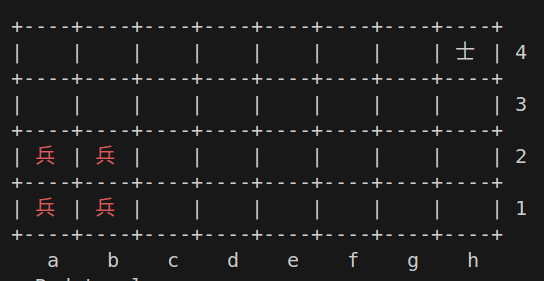
\includegraphics[totalheight=6cm]{board.png}
\end{figure}
如上圖所示,當所有紅子集中時,algorithm \ref{alg:min_move_estimate1}取到的所有邊都將是紅子間計算得出,導致即使右上角的士正確往左下移動時,algorithm \ref{alg:min_move_estimate1}的估計依然不會減少,失去作為heuristic的效果。

因此 algorithm \ref{alg:min_move_estimate2}加入跳過重複點的機制後,可以保證至少有一條邊是取自黑子->紅子,對上述問題有相當程度的改善。

以下為兩種heuristic在task 3-1至task 3-3的執行結果


\begin{table}[!h]
    \begin{tabular}{c c c c}
        Heuristic & 3-1 & 3-2 & 3-3 \\
        \hline
        algorithm \ref{alg:min_move_estimate1} & \\
        algorithm \ref{alg:min_move_estimate2} & $8\times 10^{-4} / 452$ & 1.13 / 3220270 & 4.80 / 13496393
    \end{tabular}
    \caption{performance(time / heuristic calls)}
\end{table}

% 首先,我們註解掉DFS\ref{DFS}中的line 11與line 16,禁用record與is\_visited功能,兩種heuristic


\subsection{record}


\begin{table}[!h]
    \begin{tabular}{c c c c}
        Heuristic & 3-1 & 3-3 & SH-3\\
        \hline
        without record & $8\times 10^{-4} / 452$ / 3916  & 4.80 / $1.3\times 10^8$ / 3840 & 388 /$1.1\times 10^9$ / 4028\\
        with record & $0.004 / 445/3884$  & $0.006 / 5917 / 4168$ & 0.08/ 89156/ 4844
    \end{tabular}
    \caption{performance(time / heuristic calls / memory used)}
\end{table}

\end{document}